% This is a comment.
% the region directly below this comment, up till the command \begin{document} is known as the 'preamble'
% basic setup
\documentclass{article}
\usepackage[english]{babel}
\usepackage[utf8]{inputenc}

% for mathematics
\usepackage{amsmath}
\usepackage{amsthm}
% define theorems, lemmas, etc
\newtheorem{theorem}{Theorem}
\newtheorem{lemma}{Lemma}
\newtheorem{corollary}{Corollary}
\newtheorem{definition}{Definition}
\newtheorem{example}{Example}
\usepackage{amssymb}

% for adjusting margins
\usepackage{geometry}
\geometry{
	a4paper,
 	left=26mm,
 	right=20mm,
 	top=33mm,
 	bottom=38mm
}

% for introducing urls
\usepackage{url}

% for colored text
\usepackage{color}

% for creating lists
\usepackage{enumerate}

% for import graphics
\usepackage{graphicx}

% include algorithm package
\usepackage[]{algorithm2e}

% change font to times new roman
%\usepackage{times}

% add padding to in between paragraphs
\setlength{\parskip}{1em}

% eliminate indent at start of paragraph
\setlength\parindent{0pt}

% title details
\title{QF4102 Financial Modelling and Computation Assignment 1}
%\date{}
\author{G01 Wang Zexin, Chen Penghao}

%~~~~~~~~~~~~~~~~~~~~~~~~~~~~~~~~~~~~~~~~~~~~~~~~~~~~~~~~~~~~~~~~~~~~~~~~~~~~~~
\begin{document}

% insert title
\maketitle
% make a new page
\newpage

\section{European down-and-out call option}
\subsection*{\emph{Statement of the problem}}
Write a Matlab function for the exact solution of a European down-and-out call option. Your function must be able to \textbf{work with the initial underlier price $S_{0}$ in a vector form}. 

Obtain the European down-and-out option values for time to maturity $\tau = 0.5$ year, strike price $S_0 = \$6.5$, underlier's volatility $\sigma = 30\%$, dividend yield $q = 0\%$, and risk free rate $r = 2\%$, and barrier $H = \$7$ for original prices of the underlier from $\$7$ to $\$10$ in increments of $\$0.1$. 

Obtain also the prices of European down-and-out option for the case when $H = \$6$, as well as the prices of European vanilla call option, with the same set of values of $(\tau, S_0, \sigma, q, r)$. Plot all three set of values from European down-and-out option with barrier $H = \$7$ and $H = \$6$, and European vanilla call option, on the same graph.

Implement the binomial tree method for European down-and-out option, fixing $S_0 = \$8$, $H = \$6$, and compute the option values $C_{do}^{N}$ for $N = 210, 211,...,250$. Plot the error $C^{N}_{do} - C_{do}$ against the values of $N$. Obtain the two values of $N$ that yields the minimum erors.

\subsection{Description of work done}
Using the formula defined on the assignment problem description, we can develop the following algorithm to first calculate the theoretical European down-and-out call option values for the different strike prices $S_0$.

\begin{algorithm}[H]
 \label{theoretical-do}
 \KwData{$S_0, q, H, X, \tau, r, \sigma$}
 \KwResult{$C_do$, Option Premium}
 $\lambda = \dfrac{(r - q)}{\sigma ^ 2}- 0.5$\;
 $y = \dfrac{\log{[H ^ 2/(XS_0)]}}{\sigma\sqrt{\tau}} + \lambda\sigma^2\tau$\;
 $x_1 =\dfrac{\log{S_0/H}}{\sigma\sqrt{\tau}} + \lambda\sigma^2\tau$\;
 $y_1 =\dfrac{\log{H/S_0}}{\sigma\sqrt{\tau}} + \lambda\sigma^2\tau$\;
 $d_1 =\dfrac{\log{(S_0/X)} + (r-q+\sigma^2 / 2)\tau}{\sigma\sqrt{\tau}}$\;
 $d_2 = d_1 - \sigma\sqrt{\tau}$\;
 $C = S_0e^{-q\tau}N(d_1) - X e^{-r\tau}N(d_2)$\;
 \eIf {$H \leq X$} {\textsl{•}
    $C_do = C - S_0e^{-q\tau}\left(\dfrac{H}{S_0}\right)^{2\lambda}
      + N(y-\sigma\sqrt{\tau})Xe^{-r\tau}\left(\dfrac{H}{S_0}\right)^{2\lambda-2}$\;
  }{$C_do = S_0N(x_1)e^{-q\tau}
      - Xe^{-r\tau}N(x_1-\sigma\sqrt{\tau})
      - N(y_1)S_0e^{-q\tau}\left(\dfrac{H}{S_0}\right)^{2\lambda} 
      + N(y_1-\sigma\sqrt{\tau})Xe^{-r\tau}\left(\dfrac{H}{S_0}\right)^{2\lambda-2}$\;
  }
\caption{Algorithm for pricing European down-and-out option}
\end{algorithm}

\newpage

Then we move on to develop the BTM algorithm for European down-and-out option:

\begin{algorithm}[H]
 \KwData{$S_0, q, H, X, \tau, r, \sigma$}
 \KwResult{$C_do$, Option Premium}
 $\Delta t = \tau / N$\;
 $\Delta x = \sigma \sqrt{\Delta t}$\;
 $u = e^{\Delta x}$\;
 $d = \dfrac{1}{u}$\;
 $p = \dfrac{e^{(r-q)\Delta t} - d)}{u - d}$\;
 Initialization\;
 \For {$i = 0$ to $N$} {
  $V_{N}^{i} = \max(S_0u^{2j - N} - X, 0)$\;
 }
 \For {$n = N-1, N, ... , 1, 0$} {
  \texttt{\% Get the boundary value of j}\;
  $b_j =\left \lfloor \dfrac{\log([H/S0])}{2 \Delta x}+ \dfrac{n}{2}\right\rfloor$\;
 	\For {$j = 0, 1, ... , N$} {
 		\eIf{$j > b_j$}{
 			$V_{n}^{j} = e^{-r\Delta t}(p V^{j+1}_{n+1} + (1-p)V^{j}_{n+1})$\;
 		}{$V_{n}^{j} = 0$\;}
 	}
 }
\caption{Algorithm for pricing European down-and-out option}
\end{algorithm}

We then move on to find the error between option value obtained via BTM and the theoretical option value. Fixing $S_0 = 8$ and $H = 6$, with other parameters $(q, X, \tau, r, \sigma)$ remaining the same, we first generate an array that contains the BTM down-and-out option values with time steps from 210 to 250. We then find the theoretical down-and-out option values calculated using \textbf{Algorithm 1} for the same set of parameter $(S_0, q, H, X, \tau, r, \sigma)$. Minus off this value to the array obtained before, to get the errors.

We then locate the index of the entry that has the smallest value, plus $209$ to get the number of time steps. Then we find the second minimal in the array and similarly plus back $209$ to obtain the number of time steps. The resuls turns out to be $217$ and $239$.

\newpage

\subsection{Comments on plot of option prices against current underlier price}
We first obtain the plot of option prices against the current underlier price.
\begin{figure}[htbp!]
	\centering
	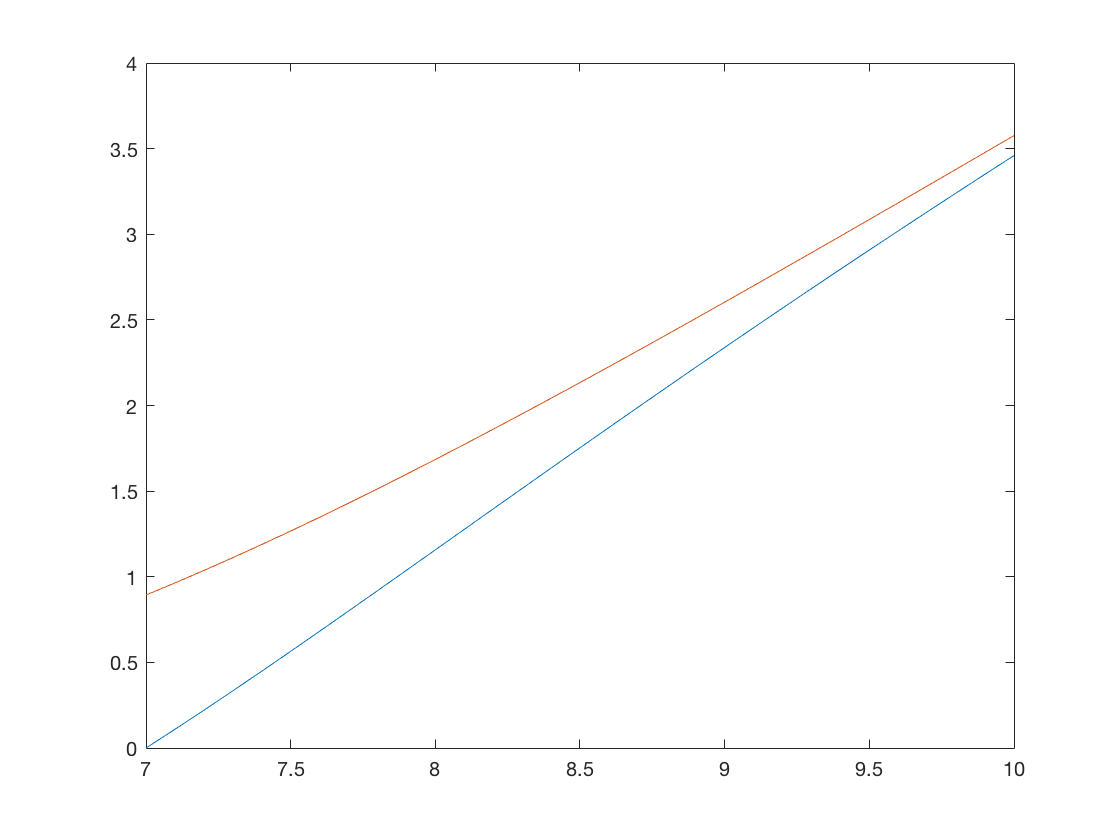
\includegraphics[scale=0.3]{A1_1_plot.png}
	\caption{Prices of down-and-out and vanilla call option against current underlier price}
\end{figure}

From the plot, we can observe that at lower values of $S_0$ the down-and-out option premium is having a larger deviation from the vanilla call option. For the down-and-out option with $H = \$7$, when $S_0=7$, it has a value of $\$0$, and the down-and-out option with $H = \$6$ is having a value of approximately $\$0.75$, while the vanilla option is having a value of near $\$1$. On the contrary, at larger values of $S_0$, the deviation appear to get smaller - the option premium for both down-and-out options converge to the European vanilla call option at large $S_0$. 

This is because as $S_0$ goes up, it has less possibility to fall into a price state that is below the threshold, thus less 0 value in the tree nodes. Hence in the backward iteration stage, we have less difference between the payoff of the down-and-out option and the vanilla option due to the presence of less zeros. Hence, The value at the original time point will be more similar to that of a European vanilla call option.

When we compare across different values of $H$, we can easily observe that the plot of the down-and-out option value with $H=\$6$ is closer to that of the European vanilla call option, compared to the plot of option premium of the down-and-out option with $H = \$7$. The reason is similar to that of the previous case, where if we set the barrier lower, there is less likelihood that the stock price will change and fall below the threshold. Thus, there are less zeros in the binomial tree nodes, and thus the option premium in period 0 is less affected by the barrier, hence more similar to the European vanilla option.

\newpage

\subsection{Comments on plot of computation errors using BTM against theoretical values}
\begin{figure}[htbp!]
	\centering
	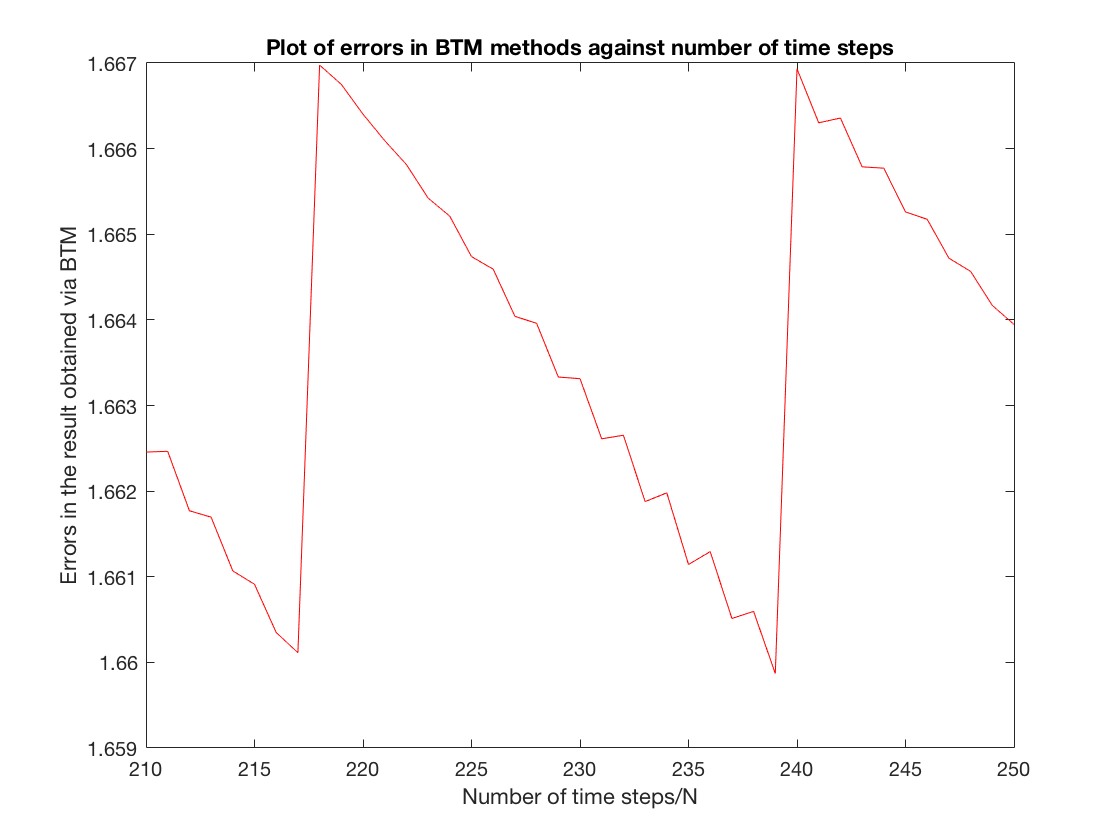
\includegraphics[scale=0.3]{A1_4_plot.PNG}
	\caption{Prices of European down-and-out call against number of time intervals}
\end{figure}

Starting with $N = 210$, the error in the results obtained start decreasing from 1.66225, and reaches a minimum point at 1.66 when $N = 217$. Then it sharply increase to its maximum value at 1.667 when $N = 218$, and decrease in a zig-zag manner from $N = 218$ to $N = 239$, where it reaches its minimum point again. This time, the minimum error is slightly lower than the one we obtained when $N = 217$. Then at $N = 240$, the error sharply increase again to slightly lower than 1.667. Hence, we observe a strong cyclic behaviour plus a less trivial general decreasing trend.

And in the range of $H = 210$ to $217$, $H = 217$ to $239$, and $H = 240$ to $250$, the shape of the plot appear to have tooths. The error does not decrease smoothly with constant drops, but rather, it may first decrease in a smaller amount, or even increase by a small ammount, then devrease drastically in the next movement. The size of the tooths is increasing in the range between $217$ and $239$.

\begin{figure}[htbp!]
	\centering
	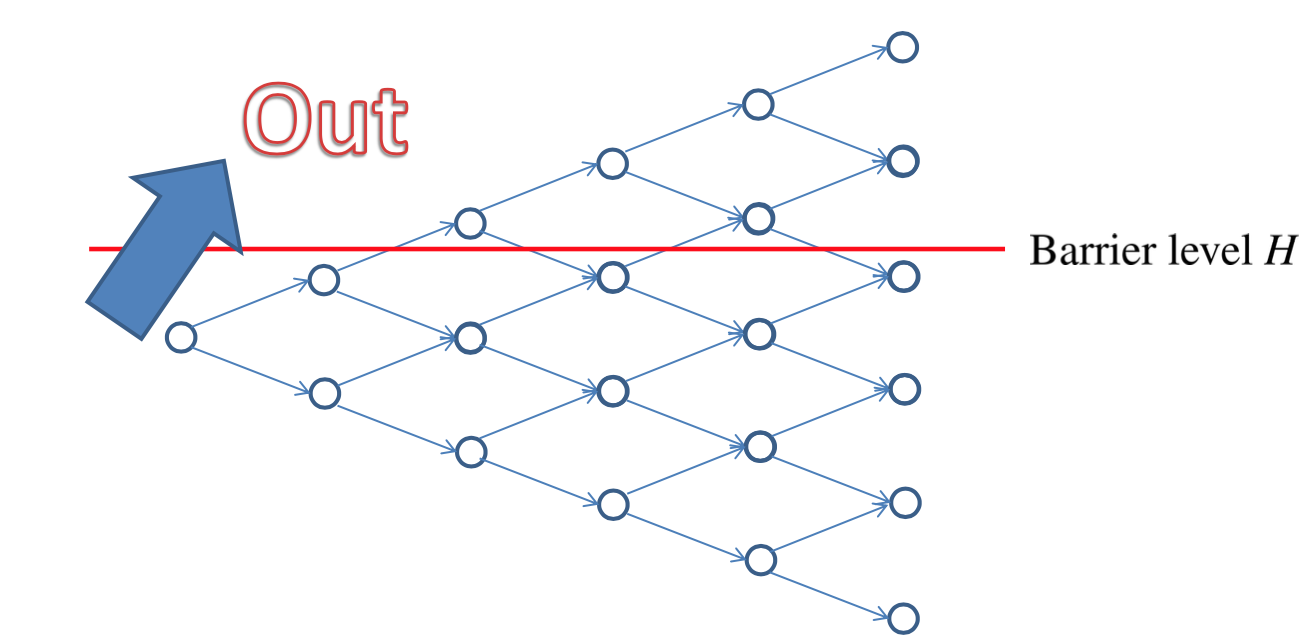
\includegraphics[scale=0.4]{Lattice_lecturenotes.PNG}
	\caption{Screenshot of lecture notes on up-and-out barrier option}
\end{figure}

As we observe from the lecture notes illustration, if we increase the time step, the original tree nodes will make a movement downwards due to decrease in length in the tree edges - since the total length is fixed for the entire tree. As the barrier is not shifted, we can observe that the periodic movement is generated by the barrier periodically becoming very close to one of the level of nodes, so that the error generated when setting the price corresponding to these nodes into zero will be minimized.

\subsection{Values of $N$ that minimizes the errors}
The two values of $N$ are \textbf{217} and \textbf{239} respectively.

\newpage

\section{European floating strike lookback put option}
\subsection*{Statement of the problem}
Write a Matlab function that implements version 1 of the single-state variable binomial tree method for approximating prices of a European floating strike lookback put option (newly issued) with $0.5$ year to maturity, current underlying price of \$1, volatility of $40\%$, dividend yield of $2\%$ and risk free rate of $4\%$. Obtain option value estiamtes for number of time steps $N$ being $200$ to $20000$ in increments of $200$. Obtain a graph of these option values versus $N$.\\
Write also a Matlab function to price European floating strike lookback put option (not newly issued). Test with same parameters with running max of \$$1.3$.

\subsection{Newly issued European floating strike lookback put options}
For the floating strike type of lookback options, we can change from a two-state model to single-state model. We make use of this property $V(A_{t},S_{t},t) = S_{t}V(\frac{A_{t}}{S_{t}}, 1, t)$, and use the new symbol $x_{t} = \ln(\frac{A_{t}}{S_{t}})$ to represent the current state on the binomial tree. Value of the option can thus be represented by $W(x_{t}, t) = \frac{V(exp(x_{t}), 1, t)}{S_{t}}$.\\
Since in this case we are only interested in the $A_{t}$ being the maximum value of underlying over time, the binomial updates of $A_{t}$ can be simplied as:
\begin{equation}
  A_{t}=
  \begin{cases}
    A_{t-1}, & \text{if}\ S_{t} = dS_{t-1} \\
    \max(A_{t-1}, S_{t}), & \text{otherwise}
  \end{cases}
\end{equation}
Furthermore, we use this upon the binomial updates of $x_{t}$:
\begin{equation}
  x_{n}^{k}=
  \begin{cases}
    x_{n-1}^{\frac{k+1}{2}} + {^{\Delta}x}, & \text{if}\ k \text{ is odd} \\
    \max(x_{n-1}^{\frac{k}{2}} - {^{\Delta}x}, 0), & \text{otherwise}
  \end{cases}
\end{equation}
where ${^{\Delta}x} = \sigma \sqrt{^{\Delta}t}$
The binomial update equation for $W(x_{n}^{k}, t_{n})$ is:
$$ W(x_{n}^{k}, t_{n}) = \exp(-r{^{\Delta}t})[puW(x_{n+1}^{2k}, t_{n+1}) + (1-p)dW(x_{n+1}^{2k+1}, t_{n+1})] $$
\begin{algorithm}[H]
 \KwData{$r, \sigma, S_{0}, \tau, N, q$}
 \KwResult{$p_{0}$, Option Premium}
 Initialization\;
 $N = \frac{T}{\delta t}$\;
 $x_{n}^{k} = k{^{\Delta}x}$\;
 Set the boundary conditions\;
 \For {i = $\max(j-N, 0)$ \dots $j+N+1$} {
  $W_{N}^{i} = \exp(x_{N}^{i}) - 1$\;
 }
 \For {n = N-1, N-2, \dots 0} {
  \If {$j - n \le 0$} {
    $W_{n}^{0} = exp(-r{^{\Delta}t})[puW_{n+1}^{0}+(1-p)dW_{n+1}^{1}]$\;
  }
  \For {k = $\max(j-n,1), \dots, j + n + 1$} {
    $W_{n}^{k} = exp(-r{^{\Delta}t})[puW_{n+1}^{k-1}+(1-p)dW_{n+1}^{k+1}]$\;
  }
 }
 $p_{0} = S_{0}W_{0}^{0}$\;
\caption{Algorithm for pricing newly issued floating strike lookback put}
\end{algorithm}
\newpage

\subsection{Previously issued European floating strike lookback put options}
In the previous case we could take advantage of the characteristic of lookback option in which all the maximum values correspond to the potential stock prices in the binomial tree. However in this case, since the option is not newly issued and we may have a previous running max which does not correspond to any of the potential stock prices, we cannot use the single state variable to fully represent both the current stock price and the running max. Therefore the following adjustment is needed:
\begin{itemize}
	\item Compare $\tilde{A}$ and $S_{0}$, if $\tilde{A}$ is smaller, treat this like a newly issued lookback option and use the previous case's algorithm
	\item let $x_{0} = \ln \frac{\tilde{A}}{S_{0}}$
	\item Determine for an integer $j$ such that $j{^{\Delta}x} < x_{0} < (j+1){^{\Delta}x}$
	\item Grow two separate linear trees from $x_{0}^{j}$ and $x_{0}^{j+1}$
	\item Perform the backward time binomial updates
	\item Interpolate between two option values at the roots to obtain option premium
\end{itemize}
Below is an algorithm developed based on this idea:\\
\begin{algorithm}[H]
 \KwData{$r, \sigma, S_{0}, \tau, N, q, \tilde{A}$}
 \KwResult{$p_{0}$, Option Premium}
 Initialization\;
 let $x_{0} = \ln \frac{\tilde{A}}{S_{0}}$ be the initial  of the single state\;
 Choose integer $j$ such that $j{^{\Delta}x} < x_{0} < (j+1){^{\Delta}x}$\;
 $N = \frac{T}{\delta t}$\;
 Set the boundary conditions\;
 \For {i = $\max(j-N, 0)$ \dots $j+N+1$} {
  $W_{N}^{i} = \exp(x_{N}^{i}) - 1$\;
 }
 \For {n = N-1, N-2, \dots 0} {
  \If {$j - n \le 0$} {
    $W_{n}^{0} = exp(-r{^{\Delta}t})[puW_{n+1}^{0}+(1-p)dW_{n+1}^{1}]$\;
  }
  \For {k = $\max(j-n,1), \dots, j + n + 1$} {
    $W_{n}^{k} = exp(-r{^{\Delta}t})[puW_{n+1}^{k-1}+(1-p)dW_{n+1}^{k+1}]$\;
  }
 }
 $p_{0}$ is approximated by interpolating between $S_{0}W_{0}^{j}$ and $S_{0}W_{0}^{j+1}$\;
\caption{Algorithm for pricing not newly issued floating strike lookback put}
\end{algorithm}
\newpage

\subsection{Analyze, compare and comment on the results}
From Figure 3, we can easily observe that as the number of time steps used in the binomial tree method slowly increases from $200$ to $20000$, the prices obtained for the newly issued floating strike lookback put option monotonically increases from \$$0.226$ to \$$0.2364$. The rate of increase gradually drops as the price increases, and we see this as an indication that the price obtained is converging to the true value of the option.\\[4mm]
\begin{figure}[h]
	\centering
	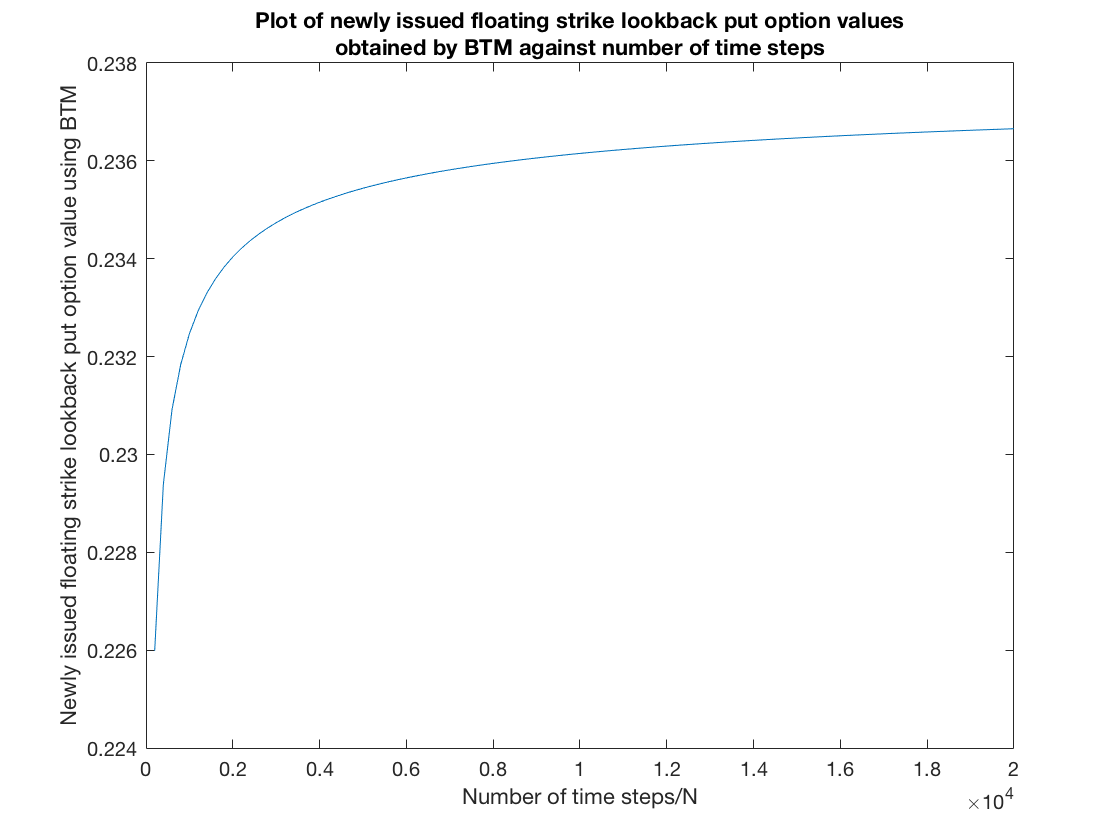
\includegraphics[scale=0.3]{A2_ni.PNG}
	\caption{Prices of newly issued floating strike lookback put against the number of time steps}
\end{figure}
If the true value is actually around $0.2364$, we should be confident that the binomial tree method with single-state modification for the European floating strike lookback put option can almost always give a good estimate of the price since the initially computed price with only $200$ time steps is very close to the true value. However, the closed-form formula does not exist for this case but once we have the finite different equations for the lookback options, the prices from FDM can be used to cross-validate the ones from binomial tree methods.\\[4mm]
Similar to the newly issued lookback put options, the prices of the previously issued lookback puts also tend from around \$$0.3466$ to \$$0.3513$, as shown in figure 4. The increase in price is also montonic and the rate of increase drops as the price increases. If we make the same assumption as for the newly issued puts, i.e. the true value lies around \$$0.3513$, we should be able to observe that value obtained from merely $200$ time steps binomial tree method is at \$$0.3466$ with only difference of \$$0.05$ from the true value.\\[4mm]
A natural question to ask may be: is this an indication that the binomial tree method may give us even more accurate value for a previously issued lookback put option? However, we shall notice that this may only attribute to the fact of having a relatively large previous running max.\\[4mm]
\begin{figure}[h]
	\centering
	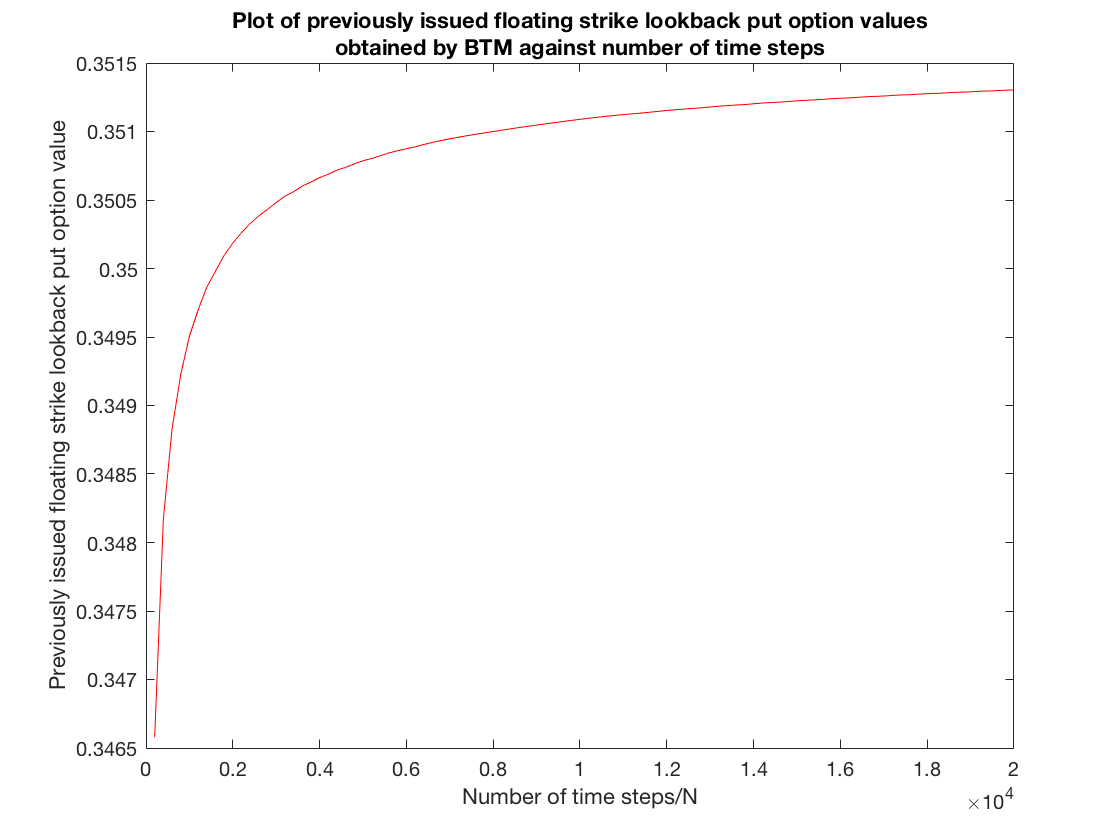
\includegraphics[scale=0.3]{A2_pi.PNG}
	\caption{Prices of previously issued floating strike lookback put against the number of time steps}
\end{figure}
We should then plot them on the same diagram and it is not hard to observe that the two price curves of these two options are very similar. Although their price levels are very different, the curvatures at various time points of the price curves are similar.
\begin{figure}[h]
	\centering
	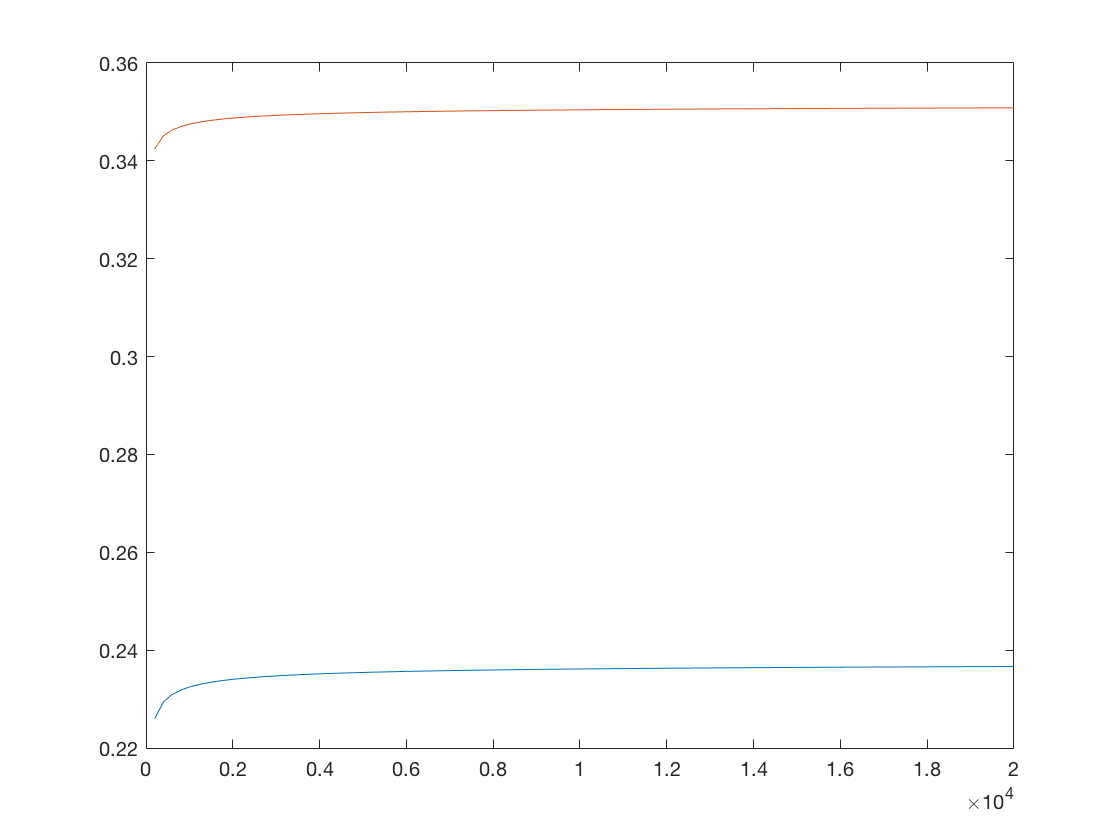
\includegraphics[scale=0.3]{A2.PNG}
	\caption{Prices of not newly issued floating strike lookback put against the number of time steps}
\end{figure}

\end{document}